\begin{frame}{ALIGN: Noisy Alt-Text at Scale}
  \begin{columns}[T,onlytextwidth]
    \column{0.52\textwidth}
      \begin{itemize}\footnotesize\itemsep0.25em
        \item \textbf{ALIGN} (Jia et al., ICML 2021): CLIP's recipe on \textbf{1.8B} image and alt-text pairs (the text a web page stores with an image).
        \item \textbf{Minimal filtering}: drop small images, alt-texts shared by over 10 images (``1920x1080''), and texts with rare tokens or under 3 or over 20 words.
        \item CLIP's pairs came from an allowlist of frequent visual concepts from English Wikipedia; ALIGN keeps the raw distribution.
        \item \textbf{Encoders}: EfficientNet-L2 and BERT-Large, from scratch; 16{,}384 pairs per batch.
        \item \textbf{Zero-shot}: ImageNet 76.4\% (CLIP 76.2\%); Flickr30K text-to-image R@1 (match ranked first) 75.7 against CLIP's 68.7.
        \item In the authors' words, ``the scale of our corpus can make up for its noise''.
      \end{itemize}
    \column{0.46\textwidth}
      \centering
      \vspace{0.4em}
      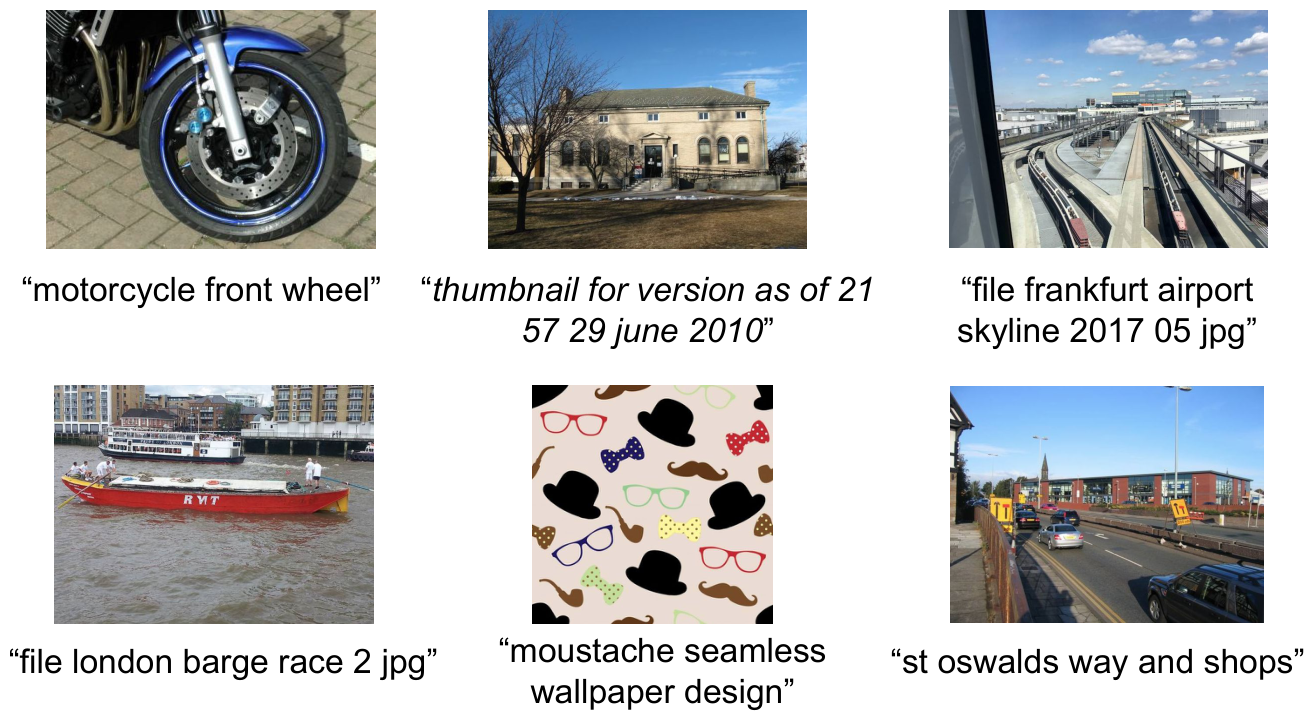
\includegraphics[width=\linewidth,height=0.46\textheight,keepaspectratio]{images/vision-language-models/align_fig2_noisy_alt_text_pairs.png}\\[0.2em]
      {\scriptsize ``Example image-text pairs randomly sampled from the training dataset of ALIGN. One clearly noisy text annotation is marked in italics.'' Jia et al., ``Scaling Up Visual and Vision-Language Representation Learning With Noisy Text Supervision,'' ICML 2021, \href{https://arxiv.org/abs/2102.05918v2}{arXiv:2102.05918v2}, Figure~2; Abstract, Secs.~2--5, Tables~1 and~4.\par}
  \end{columns}
\end{frame}

\begin{frame}{SigLIP: A Sigmoid Loss for Each Pair}
  \begin{columns}[T,onlytextwidth]
    \column{0.56\textwidth}
      \begin{itemize}\footnotesize\itemsep0.3em
        \item \textbf{SigLIP} (Zhai et al., ICCV 2023) makes every cell of the $N\times N$ matrix a yes-or-no question:
        % written as in Algorithm 1 (logits t*s+b); the Sec. 3.2 display flips the sign of b inside the exponent
        \[ \mathcal{L} = -\frac{1}{N}\sum_{i=1}^{N}\sum_{j=1}^{N}\log\sigma\big(z_{ij}\,(t\,s_{ij}+b)\big) \]
        $s_{ij}$: cosine similarity of image embedding $I_i$ and text embedding $T_j$ in a batch of $N$ pairs; $z_{ij}=1$ if $i=j$, else $-1$; $\sigma(x)=1/(1+e^{-x})$; $t=e^{t'}$: learned scale (the role of $1/\tau$); $b$: learned bias.
        \item \textbf{No normalization over the batch}: each term uses one similarity, so there are no row or column sums, and no extra pass to find the largest logit, which a stable softmax subtracts first.
        \item \textbf{Initialization} $t'=\log 10$, $b=-10$: nearly all $N^2$ pairs are negatives, so predictions start near that prior (no match) and the first updates do not overcorrect.
        \item \textbf{Ablation} (base-size model, batch 8K): ImageNet zero-shot 63.0\% with $b=-10$, 62.0\% without $b$, 61.7\% with $b=0$, 53.7\% with $b=0$ and $t'=\log 1$.
      \end{itemize}
    \column{0.42\textwidth}
      \centering
      \vspace{0.2em}
      \resizebox{\linewidth}{!}{%
      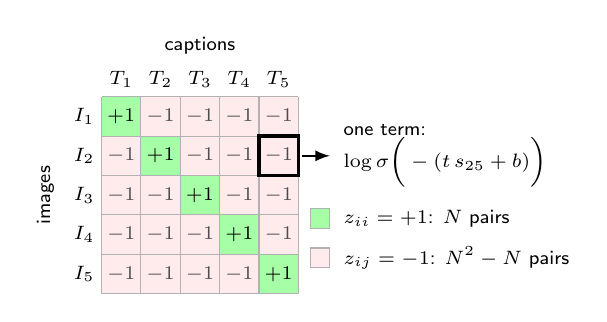
\begin{tikzpicture}[font=\sffamily\scriptsize, >=latex]
        % 5x5 layout; every cell carries its own label z_ij
        \fill[red!8] (0,-2.5) rectangle (2.5,0);
        \foreach \idx in {1,...,5}
          \fill[green!35] ({(\idx-1)*0.5},{-(\idx-1)*0.5}) rectangle ({\idx*0.5},{-\idx*0.5});
        \draw[step=0.5, gray!60] (0,-2.5) grid (2.5,0);
        \foreach \ii in {1,...,5} {
          \foreach \jj in {1,...,5} {
            \ifnum\ii=\jj\relax
              \node at ({\jj*0.5-0.25},{0.25-\ii*0.5}) {$+1$};
            \else
              \node[text=gray!60!black] at ({\jj*0.5-0.25},{0.25-\ii*0.5}) {$-1$};
            \fi
          }
        }
        \foreach \idx in {1,...,5} {
          \node at ({\idx*0.5-0.25},0.22) {$T_{\idx}$};
          \node at (-0.22,{0.25-\idx*0.5}) {$I_{\idx}$};
        }
        \node[anchor=south] at (1.25,0.42) {captions};
        \node[rotate=90, anchor=south] at (-0.48,-1.25) {images};
        \draw[very thick] (2.0,-0.5) rectangle (2.5,-1.0);
        \draw[->, thick] (2.55,-0.75) -- (2.9,-0.75);
        \node[anchor=west, align=left] at (2.95,-0.75) {one term:\\$\log\sigma\big(-(t\,s_{25}+b)\big)$};
        \fill[green!35] (2.65,-1.67) rectangle (2.9,-1.42);
        \draw[gray!60] (2.65,-1.67) rectangle (2.9,-1.42);
        \node[anchor=west] at (2.95,-1.55) {$z_{ii}=+1$: $N$ pairs};
        \fill[red!8] (2.65,-2.17) rectangle (2.9,-1.92);
        \draw[gray!60] (2.65,-2.17) rectangle (2.9,-1.92);
        \node[anchor=west] at (2.95,-2.05) {$z_{ij}=-1$: $N^2-N$ pairs};
      \end{tikzpicture}}\\[0.4em]
      {\scriptsize Each cell is its own logistic-regression example with label $z_{ij}$; no term is normalized over its row or column.\par}
      \vspace{0.4em}
      {\scriptsize Zhai et al., ``Sigmoid Loss for Language Image Pre-Training,'' ICCV 2023, \href{https://arxiv.org/abs/2303.15343v4}{arXiv:2303.15343v4}, Sec.~3.2 and Algorithm~1 (form of the loss), Sec.~4.9 and Table~4.\par}
  \end{columns}
\end{frame}

\begin{frame}{The Sigmoid Loss, Chunked Across Devices}

  {\centering
  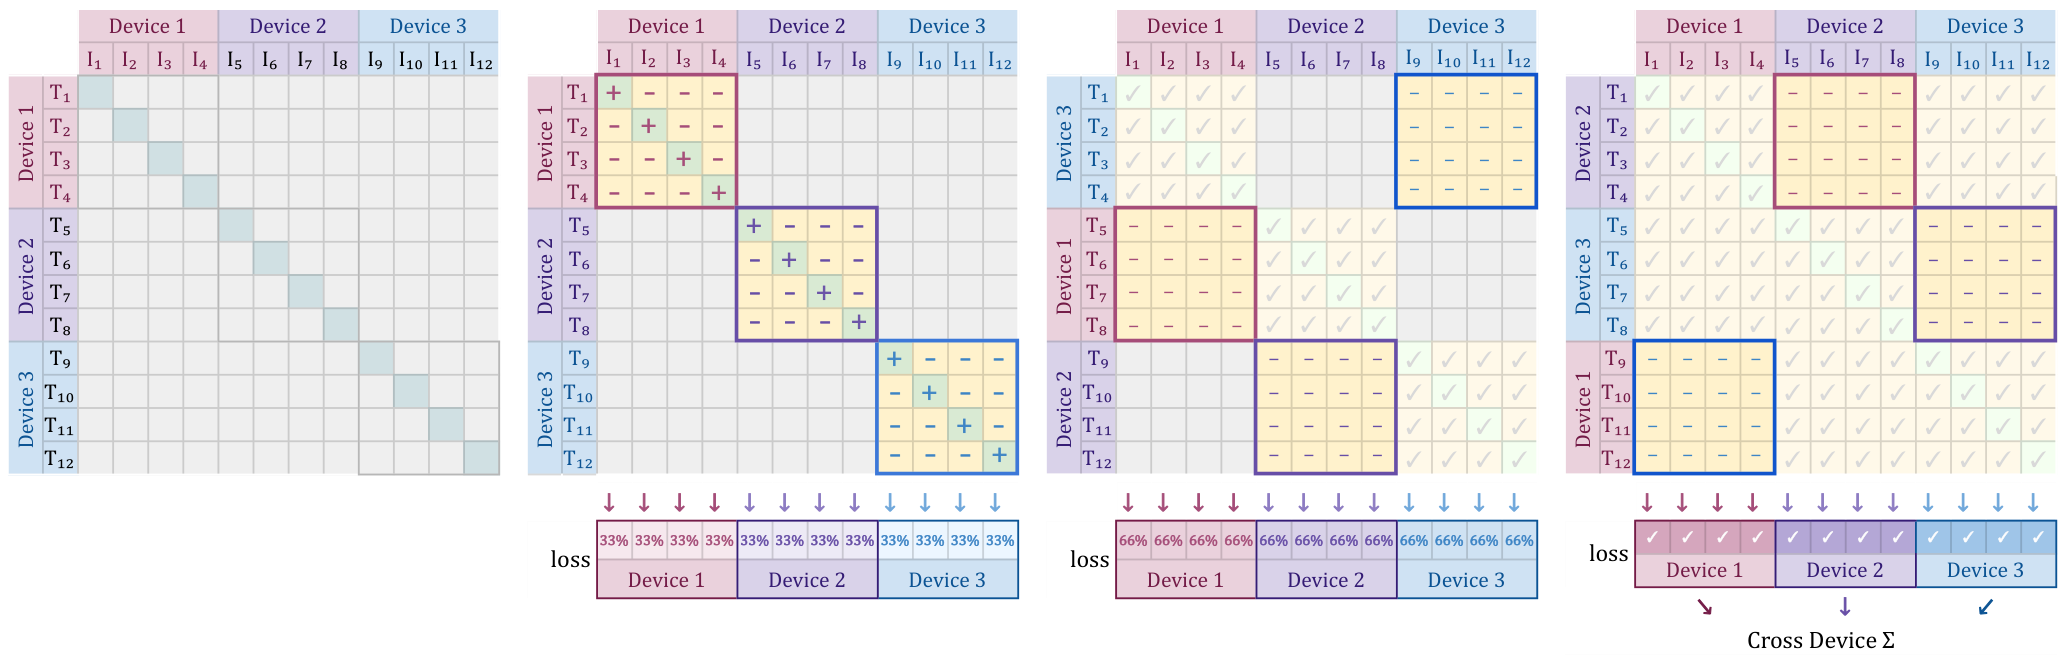
\includegraphics[width=\textwidth,height=0.62\textheight,keepaspectratio]{images/vision-language-models/siglip_fig1_chunked_loss_devices.png}\\[0.2em]
  {\scriptsize A batch of 12 on 3 devices (columns: images, rows: texts), left to right: start; local $4\times4$ blocks with the positives; texts move one device on and the new block is added; final sum across devices. Zhai et al., \href{https://arxiv.org/abs/2303.15343v4}{arXiv:2303.15343v4}, Figure~1; Sec.~3.3.\par}}
  \vspace{0.4em}
  \begin{itemize}\footnotesize
    \item Each device only ever needs its own images and one block of texts at a time, because no term looks at the rest of its row or column.
  \end{itemize}
\end{frame}

\begin{frame}{Why the Sigmoid Loss Scales}
  \begin{itemize}\itemsep0.6em
    \item \textbf{Memory}: with $D$ devices holding $m=N/D$ pairs each, a device holds one $m\times m$ block at a time and never gathers every embedding: $m^2$ entries in place of $N^2$, enough for batches above one million.
    \item \textbf{Batch size}: with a locked image tower (SigLiT: a frozen pretrained image encoder, only the text encoder trains), sigmoid beats softmax by a large margin below 16K pairs and both saturate near 32K.
    \item \textbf{Trained from scratch}, SigLIP peaks at 32K pairs while softmax needs 98K and still does not catch up; a 307K batch hurts both losses.
    \item \textbf{Cost}: SigLiT reaches 84.5\% zero-shot ImageNet on four TPUv4 chips (Google's accelerators) in two days.
  \end{itemize}
  \vspace{0.6em}
  {\scriptsize Zhai et al., \href{https://arxiv.org/abs/2303.15343v4}{arXiv:2303.15343v4}, Secs.~3.3, 4.1, 4.2 and~4.4, Figure~2 and Table~1.\par}
\end{frame}

\begin{frame}{SigLIP 2: Decoder and Self-Supervised Losses}
  \begin{columns}[T,onlytextwidth]
    \column{0.55\textwidth}
      \begin{itemize}\footnotesize\itemsep0.25em
        \item \textbf{SigLIP 2} (Tschannen et al., 2025) keeps SigLIP's architecture (swap in its weights and multilingual tokenizer) and trains it with a new recipe on alt-texts in 109 languages.
        \item \textbf{Decoder} (from LocCa, a location-aware captioner): cross-attends to the image tokens to caption, to locate phrases and to describe boxes; discarded after training.
        \item \textbf{Last 20\%}: self-distillation and masked prediction with an EMA (exponential moving average) teacher, as in DINO and iBOT, for better per-patch features.
        \item \textbf{NaFlex}: several sequence lengths at each image's native aspect ratio.
        \item SigLIP to SigLIP 2, ViT-B/16 (Base-size ViT on $16\times16$-pixel patches; L is Large) at 256 pixels: ImageNet zero-shot 76.7 to 79.1\%.
        \item SigLIP encoders are the vision towers of PaliGemma, LLaVA-OneVision and Gemma~3.
      \end{itemize}
    \column{0.43\textwidth}
      \centering
      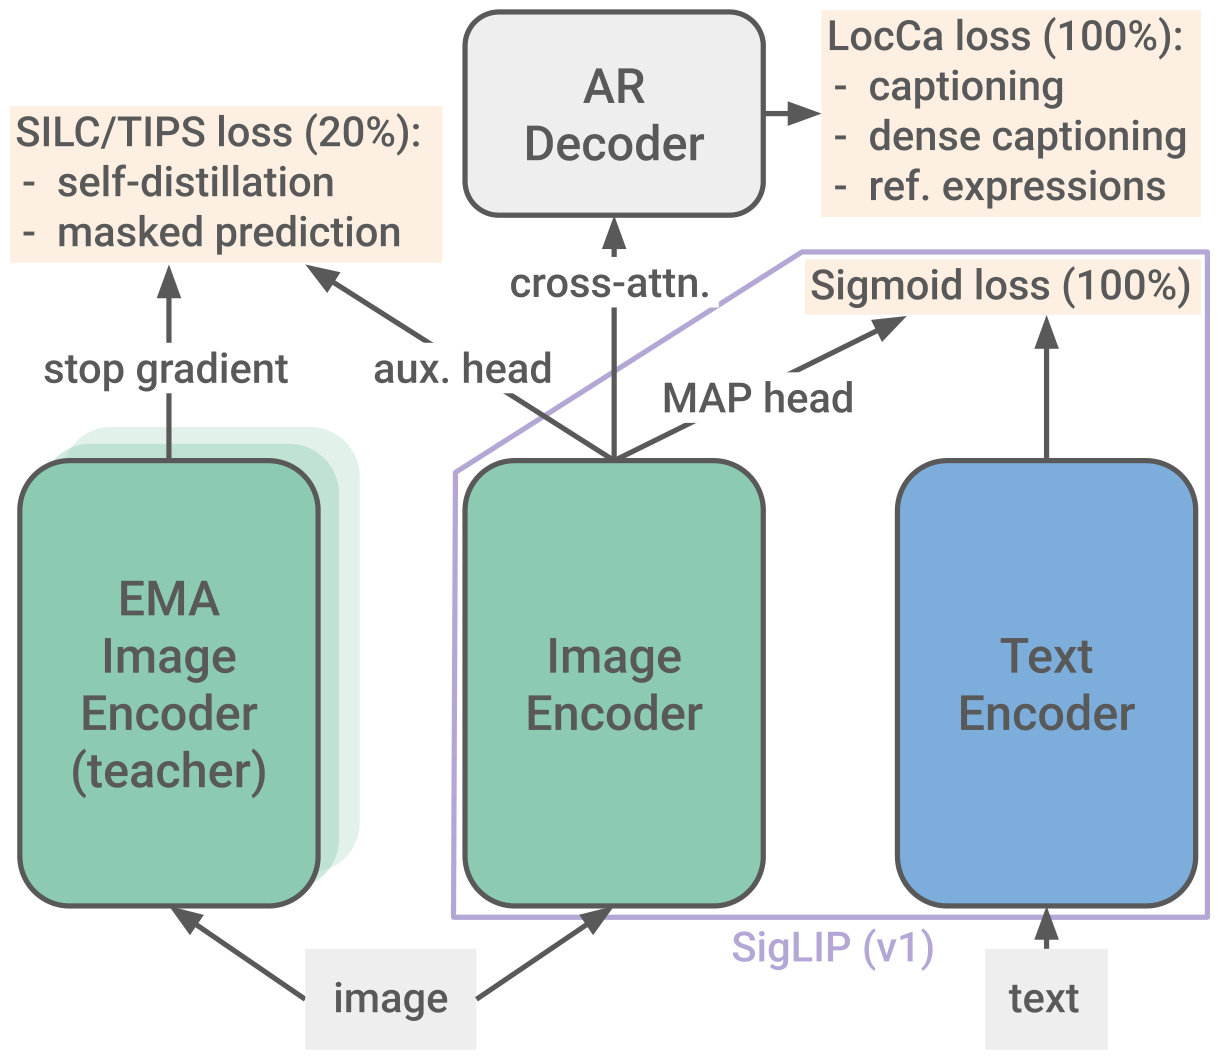
\includegraphics[width=\linewidth,height=0.50\textheight,keepaspectratio]{images/vision-language-models/siglip2_fig1_training_recipe.png}\\[0.2em]
      {\scriptsize MAP head: attention pooling of the image tokens. Tschannen et al., ``SigLIP 2: Multilingual Vision-Language Encoders with Improved Semantic Understanding, Localization, and Dense Features,'' 2025, \href{https://arxiv.org/abs/2502.14786v1}{arXiv:2502.14786v1}, Figure~1; Sec.~2 and Table~1.\par}
  \end{columns}
  \vspace{0.2em}
  {\scriptsize Vision towers: Beyer et al., PaliGemma, 2024, \href{https://arxiv.org/abs/2407.07726v2}{arXiv:2407.07726v2}, Sec.~3.1; Li et al., LLaVA-OneVision, 2024, \href{https://arxiv.org/abs/2408.03326v3}{arXiv:2408.03326v3}, Sec.~3.1; Gemma Team, Gemma~3, 2025, \href{https://arxiv.org/abs/2503.19786v1}{arXiv:2503.19786v1}, Sec.~2.1.\par}
\end{frame}

\begin{frame}{The Modality Gap}

  {\centering
  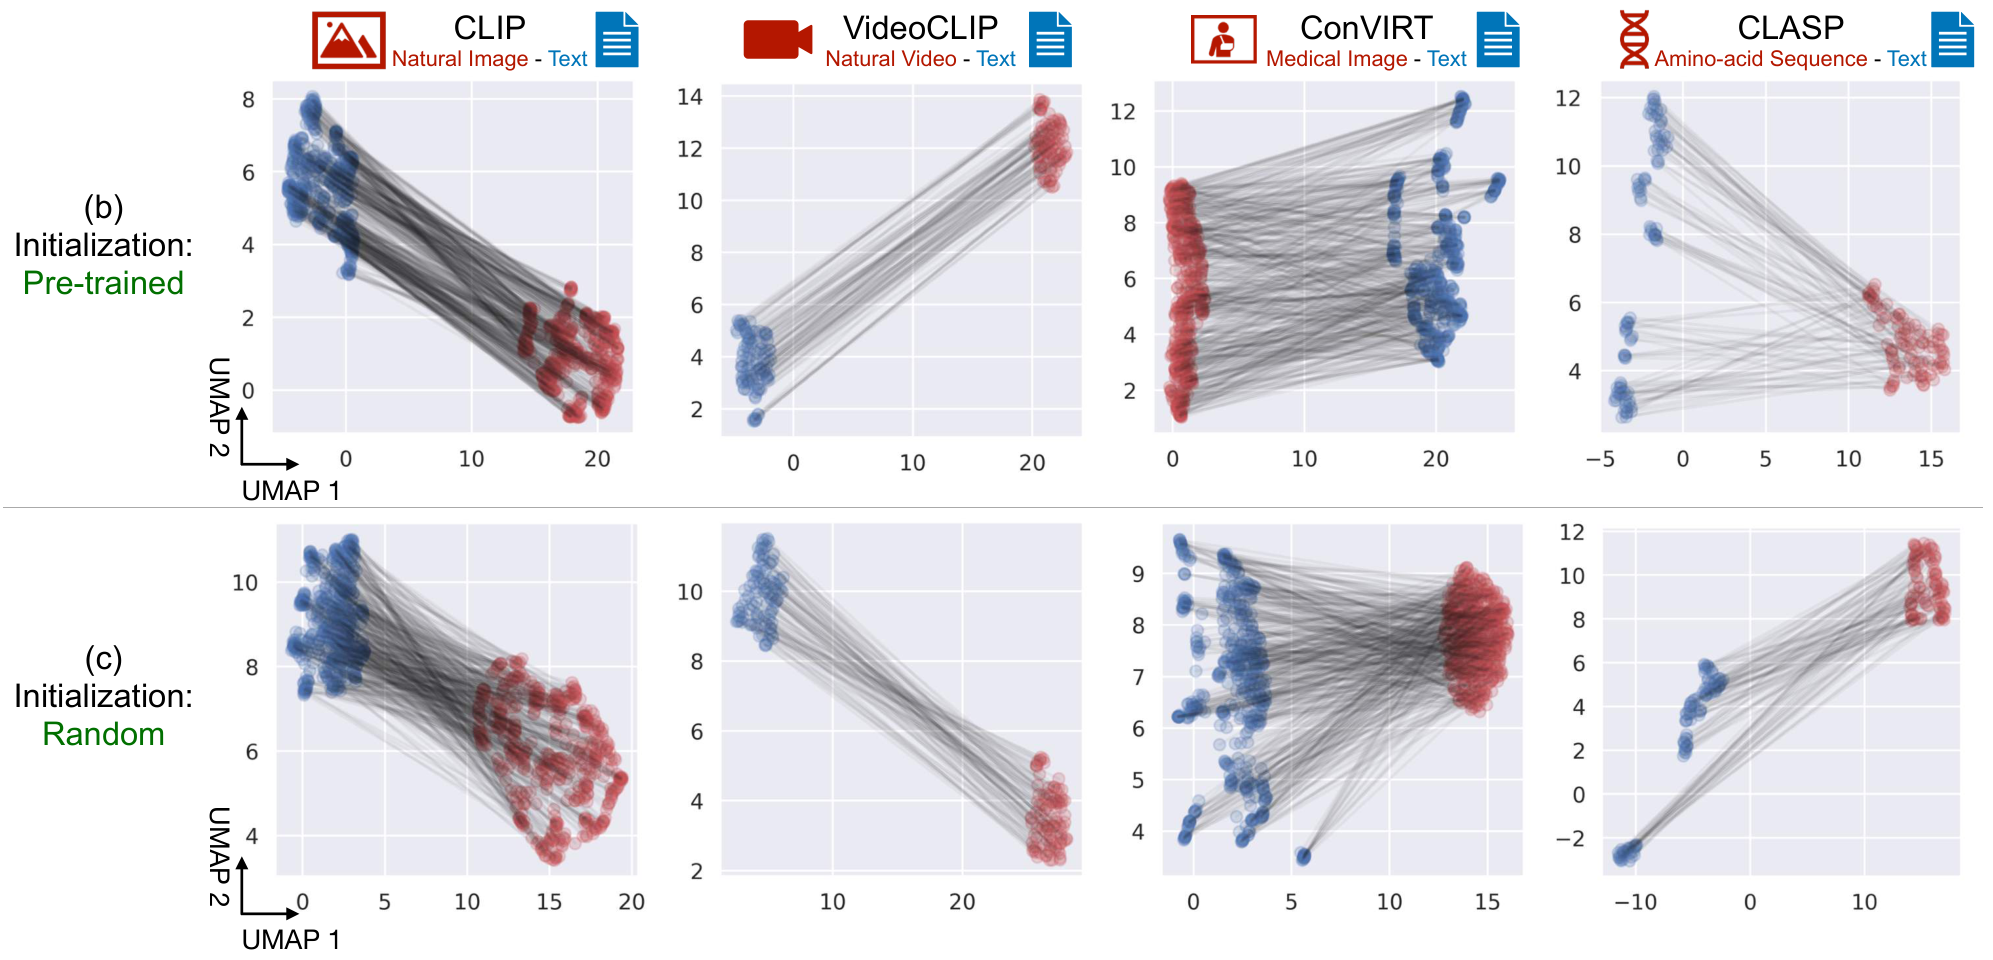
\includegraphics[width=\textwidth,height=0.64\textheight,keepaspectratio]{images/vision-language-models/modalitygap_fig1_umap_pretrained_random.png}\\[0.2em]
  {\scriptsize UMAP projections of four contrastive models (CLIP, VideoCLIP, ConVIRT, CLASP). Top row: pretrained; bottom row: randomly initialized. Red: image, video, medical-image or amino-acid embeddings; blue: text; lines join pairs. Liang et al., ``Mind the Gap: Understanding the Modality Gap in Multi-modal Contrastive Representation Learning,'' NeurIPS 2022, \href{https://arxiv.org/abs/2203.02053v2}{arXiv:2203.02053v2}, Figure~1(b,c).\par}}
\end{frame}

\begin{frame}{Where the Modality Gap Comes From}
  \begin{itemize}\itemsep0.45em
    \item \textbf{Two cones}: image and text embeddings sit in separate regions, in CLIP and in video, medical and protein models (top row of the previous figure).
    \item \textbf{From initialization}: a deep encoder maps all inputs into a narrow cone (random ResNet: mean cosine 0.99), so two encoders start apart (bottom row).
    \item \textbf{Kept by training}: at CLIP's $\tau=1/100$, closing the gap (0.82 between modality centers) raises the loss; fine-tuning at $\tau=1/10$ or $1$ shrinks it.
    \item \textbf{It matters}: shifting along the gap changed zero-shot accuracy (EuroSAT 54.1 to 56.5\%) and cut offensive labels on FairFace faces for all race groups.
    \item \textbf{In practice}: CLIP ViT-B/32 image-caption cosines mostly lie between about 0 and 0.4; use them to rank, and never compare them with text-text cosines.
  \end{itemize}
  \vspace{0.4em}
  {\scriptsize Liang et al., \href{https://arxiv.org/abs/2203.02053v2}{arXiv:2203.02053v2}, Secs.~2, 4 and~5, Tables~1--2. Cosine range: Hessel et al., ``CLIPScore: A Reference-free Evaluation Metric for Image Captioning,'' EMNLP 2021, \href{https://arxiv.org/abs/2104.08718v3}{arXiv:2104.08718v3}, Sec.~3, footnote~6; CLIPScore multiplies them by 2.5 for this reason.\par}
\end{frame}

\begin{frame}{Bag-of-Words Behavior and Hard Negatives}
  \begin{columns}[T,onlytextwidth]
    \column{0.56\textwidth}
      \begin{itemize}\footnotesize\itemsep0.3em
        \item \textbf{ARO} (Attribution, Relation, and Order; Yuksekgonul et al., ICLR 2023), over 50{,}000 cases: choose the true caption over a swapped one (``the grass is eating the horse'') or over word shuffles.
        \item \textbf{Why}: retrieval barely needs word order; with caption words shuffled, CLIP still puts a correct caption in its top 5 for 85.4\% of Flickr30K images (95.0\% intact), so pretraining need not learn order.
        \item \textbf{NegCLIP}: fine-tune on COCO with word-swapped captions as extra columns and nearest-neighbour images in the batch; CIFAR accuracy falls by at most 1 point, ImageNet from 75 to 72\%.
        \item \textbf{Winoground} (Thrush et al., CVPR 2022): 400 cases of two images and two captions with the same words reordered. Group score (all four comparisons correct): humans 85.5, CLIP ViT-B/32 8.0, chance 16.67.
      \end{itemize}
    \column{0.42\textwidth}
      \centering
      \resizebox{\linewidth}{!}{%
      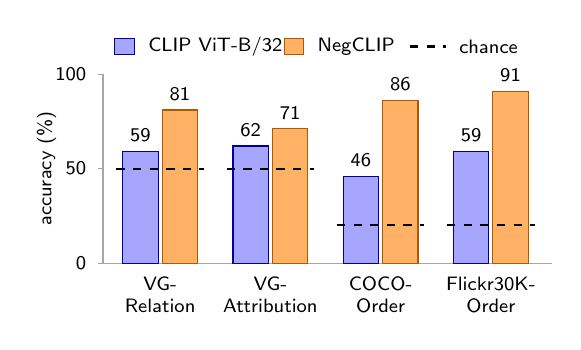
\begin{tikzpicture}[font=\sffamily\scriptsize, >=latex,
          clipbar/.style={fill=blue!35, draw=blue!60!black},
          negbar/.style={fill=orange!60, draw=orange!70!black}]
        % accuracy in percent at 0.024 cm per point (100 = 2.4 cm); data from ARO Table 6
        \draw[gray!70] (-0.15,0) -- (5.55,0);
        \draw[gray!70] (-0.15,0) -- (-0.15,2.4);
        \foreach \vv in {0,50,100} {
          \draw[gray!70] (-0.22,{\vv*0.024}) -- (-0.15,{\vv*0.024});
          \node[anchor=east] at (-0.24,{\vv*0.024}) {\vv};
        }
        \node[rotate=90, anchor=south] at (-0.62,1.2) {accuracy (\%)};
        % VG-Relation: CLIP 59, NegCLIP 81, chance 50
        \draw[clipbar] (0.10,0) rectangle (0.55,1.416);
        \draw[negbar] (0.60,0) rectangle (1.05,1.944);
        \draw[dashed, thick] (0.02,1.2) -- (1.13,1.2);
        \node[above] at (0.325,1.416) {59};
        \node[above] at (0.825,1.944) {81};
        \node[below, align=center] at (0.575,-0.05) {VG-\\Relation};
        % VG-Attribution: CLIP 62, NegCLIP 71, chance 50
        \draw[clipbar] (1.50,0) rectangle (1.95,1.488);
        \draw[negbar] (2.00,0) rectangle (2.45,1.704);
        \draw[dashed, thick] (1.42,1.2) -- (2.53,1.2);
        \node[above] at (1.725,1.488) {62};
        \node[above] at (2.225,1.704) {71};
        \node[below, align=center] at (1.975,-0.05) {VG-\\Attribution};
        % COCO-Order: CLIP 46, NegCLIP 86, chance 20
        \draw[clipbar] (2.90,0) rectangle (3.35,1.104);
        \draw[negbar] (3.40,0) rectangle (3.85,2.064);
        \draw[dashed, thick] (2.82,0.48) -- (3.93,0.48);
        \node[above] at (3.125,1.104) {46};
        \node[above] at (3.625,2.064) {86};
        \node[below, align=center] at (3.375,-0.05) {COCO-\\Order};
        % Flickr30K-Order: CLIP 59, NegCLIP 91, chance 20
        \draw[clipbar] (4.30,0) rectangle (4.75,1.416);
        \draw[negbar] (4.80,0) rectangle (5.25,2.184);
        \draw[dashed, thick] (4.22,0.48) -- (5.33,0.48);
        \node[above] at (4.525,1.416) {59};
        \node[above] at (5.025,2.184) {91};
        \node[below, align=center] at (4.775,-0.05) {Flickr30K-\\Order};
        % legend
        \draw[clipbar] (0.0,2.65) rectangle (0.25,2.85);
        \node[anchor=west] at (0.3,2.75) {CLIP ViT-B/32};
        \draw[negbar] (2.15,2.65) rectangle (2.4,2.85);
        \node[anchor=west] at (2.45,2.75) {NegCLIP};
        \draw[dashed, thick] (3.75,2.75) -- (4.2,2.75);
        \node[anchor=west] at (4.25,2.75) {chance};
      \end{tikzpicture}}\\[0.3em]
      {\scriptsize ARO accuracy (\%). VG: Visual Genome images annotated with relations and attributes; Order: the true caption against four word shuffles.\par}
      \vspace{0.3em}
      {\scriptsize Yuksekgonul et al., ``When and why vision-language models behave like bags-of-words, and what to do about it?,'' ICLR 2023, \href{https://arxiv.org/abs/2210.01936v3}{arXiv:2210.01936v3}, Abstract, Secs.~2 and~4, Tables~3 and~6.\par}
  \end{columns}
  \vspace{0.2em}
  {\scriptsize Thrush et al., ``Winoground: Probing Vision and Language Models for Visio-Linguistic Compositionality,'' CVPR 2022, \href{https://arxiv.org/abs/2204.03162v2}{arXiv:2204.03162v2}, Sec.~3 and Table~3.\par}
\end{frame}

\begin{frame}{Captioning as an Alignment Signal: CoCa}
  \begin{columns}[T,onlytextwidth]
    \column{0.58\textwidth}
      \begin{itemize}\footnotesize\itemsep0.3em
        \item \textbf{CoCa} (Yu et al., 2022) trains an image encoder and a text decoder from scratch on
        \[ \mathcal{L} = \lambda_{\text{Con}}\,\mathcal{L}_{\text{Con}} + \lambda_{\text{Cap}}\,\mathcal{L}_{\text{Cap}}, \quad \lambda_{\text{Con}}=1,\ \lambda_{\text{Cap}}=2 \]
        $\mathcal{L}_{\text{Con}}$: CLIP's loss with $\frac{1}{N}$ in place of $\frac{1}{2N}$; $\mathcal{L}_{\text{Cap}}=-\sum_t\log p_\theta(y_t\mid y_{<t},x)$, where $p_\theta$ is the decoder's probability of caption token $y_t$ given image $x$ and the earlier tokens.
        \item \textbf{Decoder}: the lower half has no cross-attention; its output at an appended [CLS] token (an extra token that summarizes the sequence) is the text embedding for $\mathcal{L}_{\text{Con}}$. The upper half cross-attends to the image and predicts the caption; one forward pass gives both losses.
        \item \textbf{ImageNet}: 86.3\% zero-shot, 90.6\% with a frozen encoder, 91.0\% fine-tuned. In a base-size ablation, adding $\mathcal{L}_{\text{Cap}}$ raised zero-shot accuracy from 70.7 to 71.6\%.
        \item The next model, BLIP, keeps the contrastive and captioning objectives and adds a matching one.
      \end{itemize}
    \column{0.40\textwidth}
      \centering
      \vspace{0.2em}
      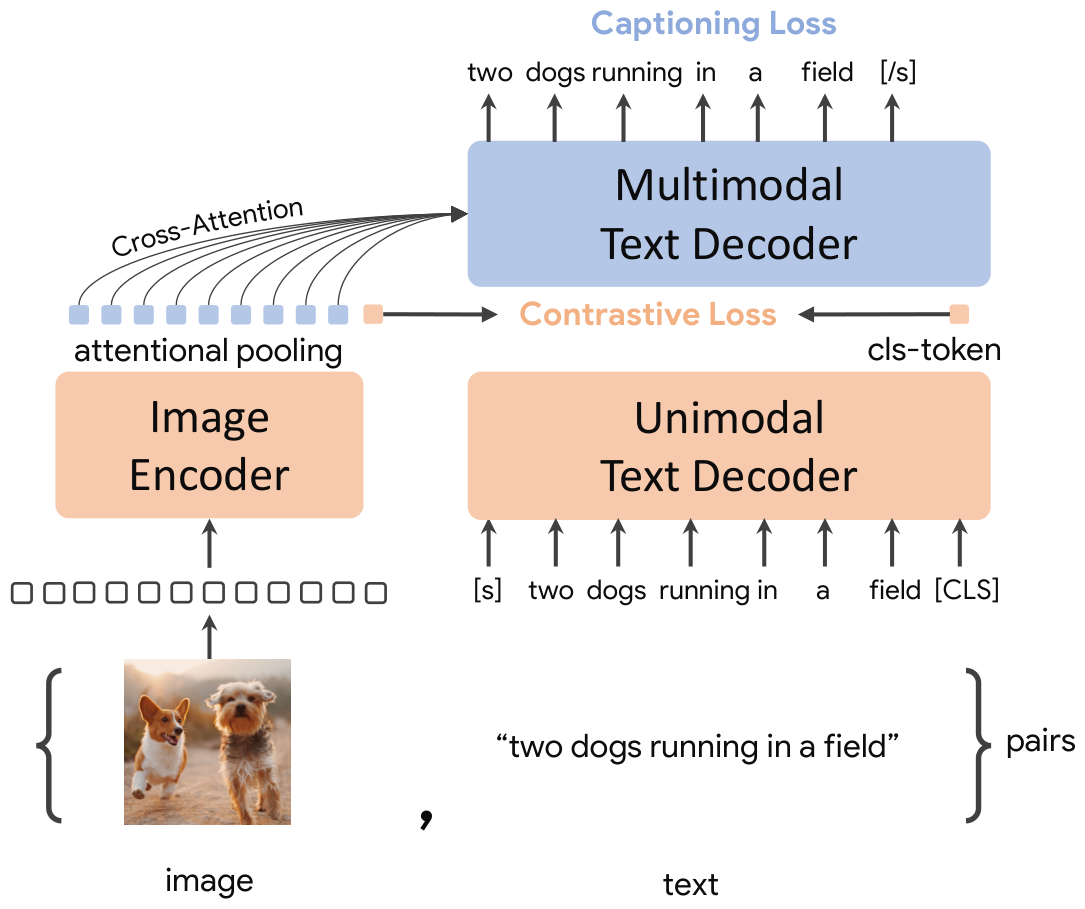
\includegraphics[width=\linewidth,height=0.46\textheight,keepaspectratio]{images/vision-language-models/coca_fig2_architecture.png}\\[0.2em]
      {\scriptsize Attentional pooling: learned queries attend over the image tokens (1 query for the contrastive embedding, 256 for the decoder). Yu et al., ``CoCa: Contrastive Captioners are Image-Text Foundation Models,'' 2022, \href{https://arxiv.org/abs/2205.01917v2}{arXiv:2205.01917v2}, Figure~2 (left half; pseudocode omitted); Secs.~3.2 and~4, Table~8.\par}
  \end{columns}
\end{frame}

\begin{frame}{Curating Image-Text Pairs: DataComp and MetaCLIP}
  \begin{columns}[T,onlytextwidth]
    \column{0.58\textwidth}
      \begin{itemize}\footnotesize\itemsep0.25em
        \item \textbf{LAION-5B}: 5.85B web pairs whose CLIP ViT-B/32 image-text cosine is at least 0.28 (0.26 if not English).
        \item \textbf{DataComp} (Gadre et al., NeurIPS 2023): fixed training code and compute; entrants compete on the data, mostly by filtering a 12.8B-pair pool (38 test sets).
        \item At the 12.8B scale the best filter adds 6.9 ImageNet points over no filtering. \textbf{DataComp-1B}: pairs in the top 30\% by CLIP ViT-L/14 score whose images also cluster near ImageNet images.
        \item \textbf{MetaCLIP} (Xu et al., 2023): keep pairs whose text contains one of 500{,}000 WordNet and Wikipedia entries, at most 20{,}000 per entry (``photo'': 54M matches, 20K kept).
        \item Without that cap, the whole 1.6B matched pool lowers ViT-B/32 from 65.5 to 61.9\%.
      \end{itemize}
    \column{0.40\textwidth}
      \centering
      {\scriptsize ImageNet zero-shot top-1 (\%); within a block the model and training compute match. WIT: CLIP's own 400M pairs.\par}
      \vspace{0.3em}
      {\scriptsize
      \begin{tabular}{@{}lr@{}}
        \toprule
        \textbf{Training data} & \textbf{ImageNet} \\
        \midrule
        \multicolumn{2}{@{}l}{ViT-L/14, 13B samples seen, same compute} \\
        WIT (0.4B) & 75.5 \\
        LAION-400M (0.4B) & 72.8 \\
        LAION-2B (2.3B) & 73.1 \\
        DataComp-1B (1.4B) & \textbf{79.2} \\
        \addlinespace[0.2em]
        \multicolumn{2}{@{}l}{ViT-B/16, CLIP's training recipe} \\
        WIT (0.4B) & 68.3 \\
        MetaCLIP (0.4B) & 70.8 \\
        MetaCLIP (1B) & \textbf{72.4} \\
        \bottomrule
      \end{tabular}\par}
      \vspace{0.3em}
      {\scriptsize Gadre et al., ``DataComp: In search of the next generation of multimodal datasets,'' NeurIPS 2023 Datasets and Benchmarks, \href{https://arxiv.org/abs/2304.14108v5}{arXiv:2304.14108v5}, Table~1, Secs.~1 and~4; Xu et al., ``Demystifying CLIP Data,'' 2023, \href{https://arxiv.org/abs/2309.16671v6}{arXiv:2309.16671v6}, Sec.~3, Tables~4--6.\par}
  \end{columns}
  \vspace{0.2em}
  {\scriptsize Schuhmann et al., ``LAION-5B: An open large-scale dataset for training next generation image-text models,'' NeurIPS 2022 Datasets and Benchmarks, \href{https://arxiv.org/abs/2210.08402v1}{arXiv:2210.08402v1}, Abstract and Sec.~3.1.\par}
\end{frame}
